\clearpage
\begin{landscape}
\begin{figure}[H]
\centering
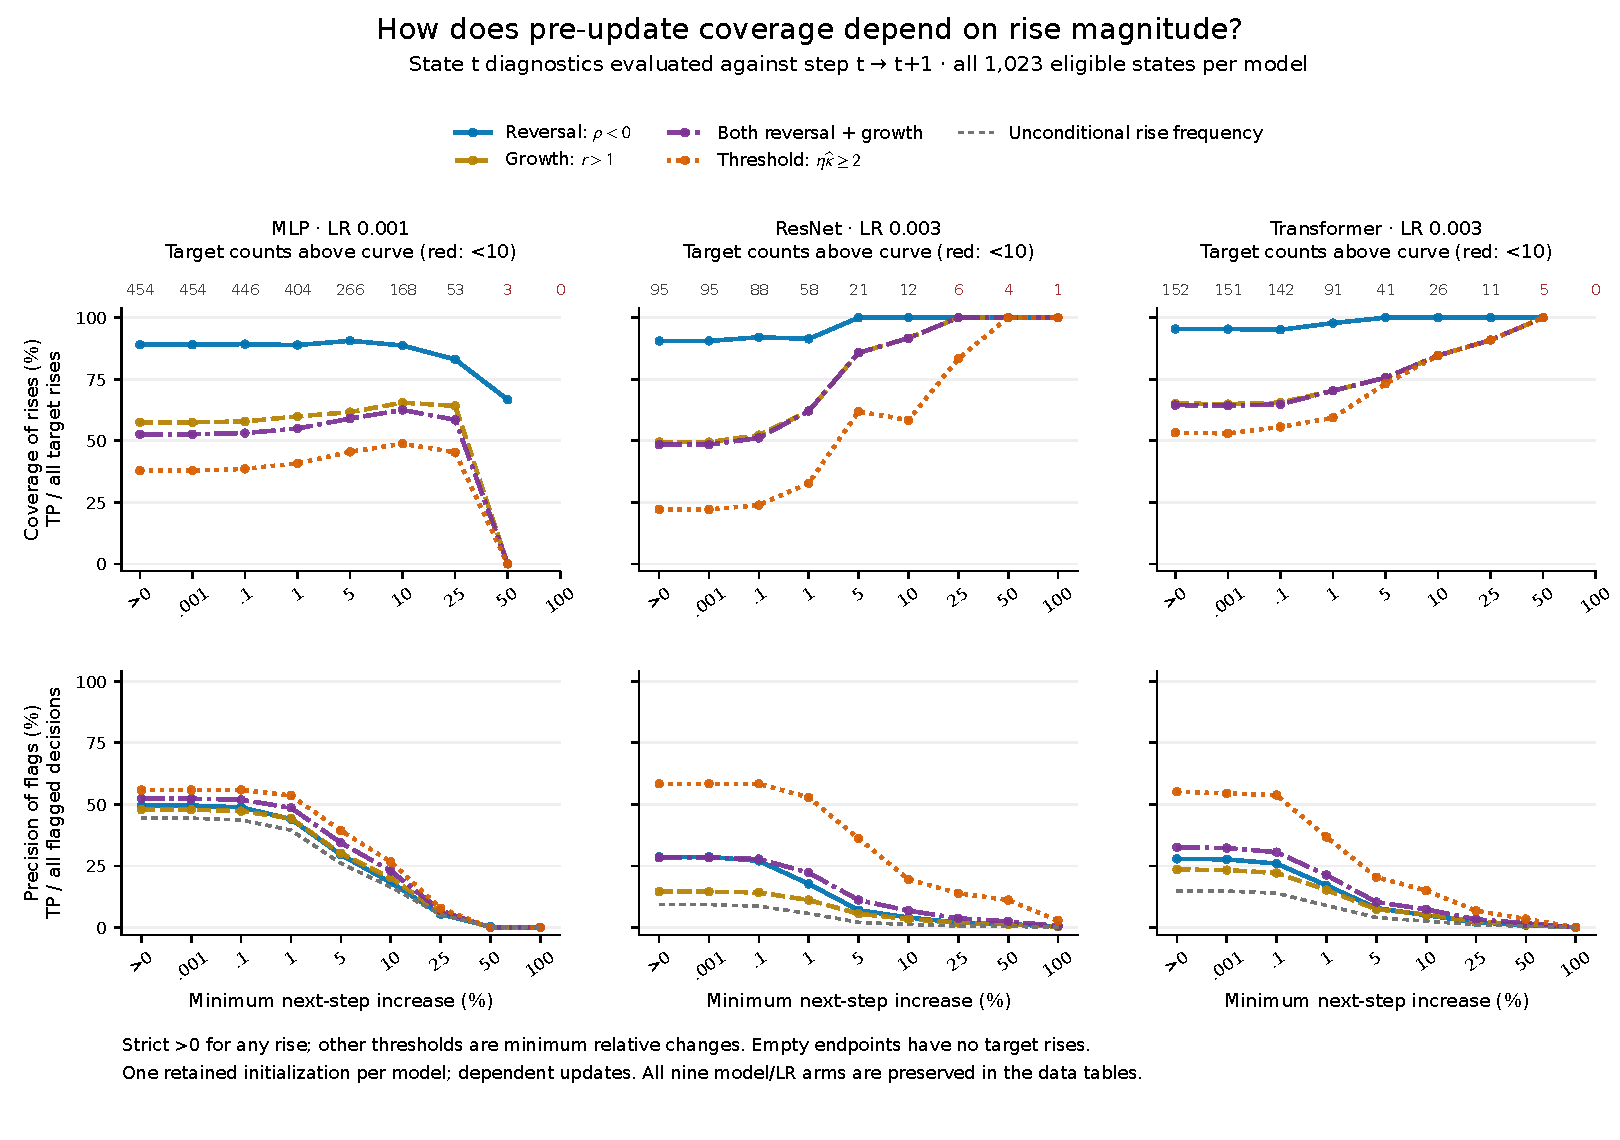
\includegraphics[page=1,width=9.6in]{figures/adam_forward_and_severity.pdf}
\caption{Coverage and precision versus minimum next-step relative loss increase. All 1,023 eligible decisions per model are retained; counts identify rare targets. Reversal, growth, their conjunction, and the projected-response threshold are compared with unconditional frequency.}
\end{figure}
\end{landscape}
\clearpage
\begin{landscape}
\begin{figure}[H]
\centering
\includegraphics[page=2,width=9.6in]{figures/adam_forward_and_severity.pdf}
\caption{Individual loss increases of at least 10 percent at each future offset. All offsets use the same 1,008 decision states. Coverage and precision describe the current flag at that offset; they are not validation of an outcome-selected lead time.}
\end{figure}
\end{landscape}
\clearpage
\begin{landscape}
\begin{figure}[H]
\centering
\includegraphics[page=3,width=9.6in]{figures/adam_forward_and_severity.pdf}
\caption{Net loss increase of at least 10 percent from the decision state to each future horizon. This target differs from an individual future step increase; common decision support is retained.}
\end{figure}
\end{landscape}
\clearpage
\begin{landscape}
\begin{figure}[H]
\centering
\includegraphics[page=4,width=9.6in]{figures/adam_forward_and_severity.pdf}
\caption{Any loss at least 10 percent above the decision-state loss within the future horizon. The target set expands with the horizon, so increasing precision must be compared with its rising base frequency.}
\end{figure}
\end{landscape}
\clearpage
\begin{landscape}
\begin{figure}[H]
\centering
\includegraphics[page=5,width=9.6in]{figures/adam_forward_and_severity.pdf}
\caption{Within-horizon increases restricted to currently non-rising decisions. This excludes an already-rising step but not necessarily an ongoing excursion. Sparse threshold support and target frequencies remain visible.}
\end{figure}
\end{landscape}
\clearpage
\begin{landscape}
\begin{figure}[H]
\centering
\includegraphics[page=6,width=9.6in]{figures/adam_forward_and_severity.pdf}
\caption{Remembered warnings for the unique next-step target. Each target is counted once; all memory widths use decisions 16--1023. Longer memory increases both coverage and the number of non-target flags.}
\end{figure}
\end{landscape}
